\chapter{Espaces de Sobolev}\label{Ch-Sobo}\index[aut]{Sobolev (Sergueï Lvovitch), 1908-1989, Russe}
\begin{abstract}
Les espaces de Sobolev sont des espaces fonctionnels.
Plus précisément, un espace de Sobolev est un espace vectoriel de fonctions muni de la norme obtenue par la combinaison de la norme~$L^p$ de la fonction elle-même ainsi que de ses dérivées jusqu'à un certain ordre.
Les dérivées sont comprises dans un sens faible, au sens des distributions afin de rendre l'espace complet.

Les espaces de Sobolev sont donc des espaces de Banach.
Intuitivement, un espace de Sobolev est un espace de Banach ou un espace de Hilbert de fonctions pouvant être dérivées suffisamment de fois (pour donner sens par exemple à une équation aux dérivées partielles) et muni d'une norme qui mesure à la fois la taille et la régularité de la fonction.

Les espaces de Sobolev sont un outil très important et très adapté à l'étude des équations aux dérivées partielles. En effet, les solutions d'équations aux dérivées partielles, appartiennent plus naturellement à un espace de Sobolev qu'à un espace de fonctions continues dont les dérivées sont comprises dans un sens classique (mais rien n'empêche d'avoir de la chance).
\end{abstract}

\medskip
\begin{histoire}%
Le \textsc{xx}\fup{e} siècle avait commencé par la thèse de Lebesgue\index[aut]{Lebesgue (Henri-Léon), 1875-1941, Français} \emph{intégrale, longueur, aire}, qui constitue vraiment le début de la théorie de la mesure.
La théorie de Lebesgue mène à l'étude des espaces~$L^p$, qui permettront, sur les traces de Hilbert,\index[aut]{Hilbert (David), 1862-1943, Allemand} Riesz\index[aut]{Riesz (Frigyes), 1880-1956, Hongrois} et Banach,\index[aut]{Banach (Stephan), 1892-1945, Polonais} l'étude des opérateurs différentiels.

\sbox{\MaBoiteAvecPhotos}{\setlength{\tabcolsep}{0pt}\scriptsize%
\begin{tabular}{cccc}
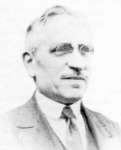
\includegraphics[height=\the\HauteurDesPhotos]{Lebesgue3}&
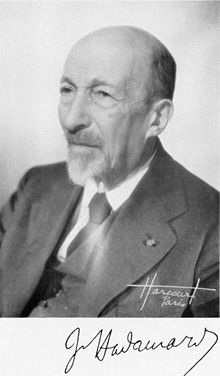
\includegraphics[height=\the\HauteurDesPhotos]{Hadamard}&
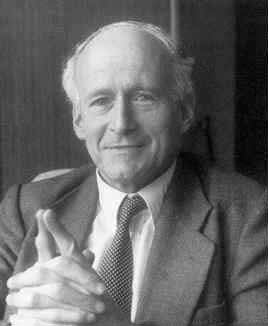
\includegraphics[height=\the\HauteurDesPhotos]{Schwartz}&
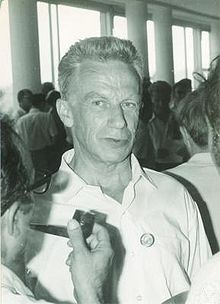
\includegraphics[height=\the\HauteurDesPhotos]{Sobolev}\\
Lebesgue &Hadamard &Schwartz &Sobolev%
\end{tabular}}
\medskip
\ImageADroite{%\ifVersionDuDocEstVincent\begin{cutout}{0}{0.50\linewidth}{0pt}{8}\else\begin{cutout}{0}{0.44\linewidth}{0pt}{8}\fi
Cauchy\index[aut]{Cauchy (Augustin Louis, baron -), 1789-1857, Français} avait publié nombre d'applications de sa théorie dans des recueils d'exercices, notamment concernant l'évaluation d'intégrales réelles, qu'il n'hésita pas à généraliser en ce qu'on appelle aujourd'hui la «valeur principale de Cauchy», un peu moins d'un siècle avant que Hadamard\index[aut]{Hadamard (Jacques Salomon), 1865-1963, Français} en ait besoin dans sa résolution des équations aux dérivées partielles dans un problème d'hydrodynamique par les «parties finies» et que Laurent Schwartz\index[aut]{Schwartz (Laurent), 1915-2002, Français} n'en vienne aux distributions.}

\medskip
L'étude des conditions de régularité des solutions des équations aux dérivées partielles permet à Sergueï Sobolev\index[aut]{Sobolev (Sergueï Lvovitch), 1908-1989, Russe} et ses continuateurs de définir ses espaces de fonctions et les théorèmes de trace en fonction des propriétés géométriques du domaine.

\medskip
Quelques mots s'imposent au sujet de la théorie des distributions.
Parmi tous les travaux ayant valus à leur auteur la médaille Fields, la théorie des distributions de Laurent Schwartz\index[aut]{Schwartz (Laurent), 1915-2002, Français} est l'une des très rares à être abordable par les étudiants dès leur premier cycle universitaire. C'est une partie de l'explication du réel engouement pour les distributions, l'autre partie étant sa puissance, sa commodité d'usage et surtout sa très grande beauté.

Si cette théorie fournit aux analystes un cadre général et un formalisme agréable pour l'étude des espaces fonctionnels et des équations aux dérivées partielles dans lesquels ils aiment à se placer, elle n'est pourtant pas indispensable.
D'une part, les spécialistes d'équations aux dérivées partielles parviennent toujours à trouver des formulations bien adaptées à leurs problèmes, en s'inspirant des idées sous-jacentes à la théorie des distributions, mais sans y avoir recours explicitement. D'autre part, on peut étudier la plupart des espaces fonctionnels intéressants sans la notion de distribution: par exemple, les espaces de Sobolev peuvent être définis en termes de  distributions, ou bien en termes de complétion de l'espace des fonctions $C^\infty$ à support compact pour des normes bien choisies. %L'équivalence de ces deux points de vue est d'ailleurs un résultat célèbre dû à Meyers et Serin.

En utilisant uniquement des espaces de Sobolev et leurs espaces duals, on peut obtenir la grande majorité des distributions que l'on rencontre en pratique: par exemple, la dérivée de la «fonction de Dirac»\index[aut]{Dirac (Paul Adrien Maurice), 1902-1984, Anglais} peut être vue comme un élément de l'espace dual des fonctions $C^1$. Plus généralement, quand on rencontre une distribution dans un problème concret, c'est presque à coup sûr un élément du dual d'un espace de Sobolev bien choisi, au moins localement. La topologie des espaces de Sobolev étant beaucoup plus simple que celle des distributions, on comprend que l'étude des espaces de Sobolev soit plus populaire et certainement plus utile en pratique. De plus, les résultats que l'on obtient en utilisant des méthodes plus terre-à-terre sont souvent meilleurs (plus constructifs, plus quantitatifs...).

Pour autant, la théorie des distributions fournit un formalisme commode et élégant, qui apporte de l'ordre dans le paysage fonctionnel, et facilite la communication entre mathématiciens d'horizons très divers. En outre, les principes qui la sous-tendent, bien plus que les théorèmes principaux, s'avèrent d'une importance capitale en pratique. Pour toutes ces raisons, une bonne familiarité avec le langage des distributions est presque indispensable à un analyste. Schwartz\index[aut]{Schwartz (Laurent), 1915-2002, Français} lui-même avait bien conscience que le principal mérite de son approche ne résidait pas dans l'introduction d'outils nouveaux, mais dans une synthèse claire et accessible de recettes multiples qui étaient, déjà auparavant, employées dans des contextes divers.
\end{histoire}
\colorblack

\medskip
\section{Distributions}\index{distribution}
Une distribution (également appelée fonction généralisée) est un objet qui généralise la notion de fonction et de mesure. La théorie des distributions étend la notion de dérivée à toutes les fonctions localement intégrables et au-delà.

\begin{histoire}
\noindent\emph{Généralisation de la notion de fonction:}\\
\sbox{\MaBoiteAvecPhotos}{\setlength{\tabcolsep}{0pt}\scriptsize%
\begin{tabular}{c}
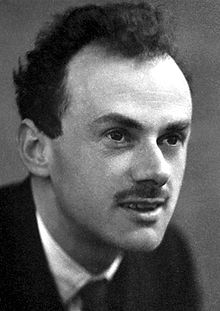
\includegraphics[height=\the\HauteurDesPhotos]{Dirac}\\
Dirac%
\end{tabular}}
\ImageADroite{%
Depuis le milieu des années 1920, les théoriciens de la physique quantique, et en particulier Dirac,\index[aut]{Dirac (Paul Adrien Maurice), 1902-1984, Anglais} utilisaient des objets étranges qu'ils manipulaient comme des fonctions. Le plus typique était la «fonction de Dirac»,\index[aut]{Dirac (Paul Adrien Maurice), 1902-1984, Anglais} mystérieuse fonction qui vaut $0$ partout, sauf en $0$ où elle vaut $+\infty$, et dont l'intégrale est égale à $1$ (en violation de toutes les règles de la théorie de l'intégration de Lebesgue). Non seulement Dirac\index[aut]{Dirac (Paul Adrien Maurice), 1902-1984, Anglais} utilisait cette fonction à des fins de calcul formel, mais encore il se permettait de la dériver à volonté, se contentant de remarquer que les dérivées successives étaient «de plus en plus singulières».\\
\indent L'utilité et le caractère intuitif de ces objets rendait presque indispensable leur incorporation dans une théorie mathématique; c'est ce qu'a réalisé la théorie des distributions. Leur interprétation est d'ailleurs très simple, et cause beaucoup moins de
maux de tête que les interrogations que l'on peut avoir sur la nature des «fonctions»
considérées par Dirac.\index[aut]{Dirac (Paul Adrien Maurice), 1902-1984, Anglais}}

\medskip
\noindent\emph{Réhabilitation de la dérivation:}\\
\sbox{\MaBoiteAvecPhotos}{\setlength{\tabcolsep}{0pt}\scriptsize%
\begin{tabular}{cc}
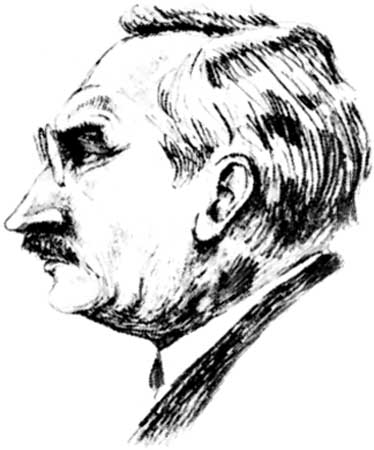
\includegraphics[height=\the\HauteurDesPhotos]{Lebesgue4}&
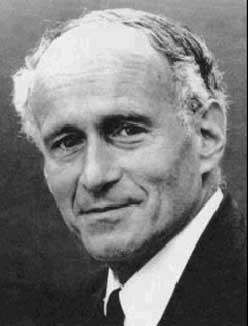
\includegraphics[height=\the\HauteurDesPhotos]{Schwartz2}\\
Lebesgue&Schwartz%
\end{tabular}}
\ImageAGauche{%
Au début du vingtième siècle, la théorie de l'intégration de Lebesgue a pris un essor rapide, et l'intégration apparaît désormais comme l'opération reine de l'analyse. La plupart des fonctions sont intégrables, alors que très peu sont dérivables. En outre, la théorie de Lebesgue montre que l'intégration est souvent une opération continue vis-à-vis de la convergence des fonctions, uniforme ou même simple (ponctuelle), alors que la dérivation est une opération grossièrement discontinue.\\
\indent
Dans la théorie de Schwartz\index[aut]{Schwartz (Laurent), 1915-2002, Français} au contraire, ces problèmes disparaîtront: à toute fonction continue on pourra associer des «fonctions dérivées» à tous les ordres, selon une notion qui prolongera celle de dérivée des fonctions continûment dérivables. De manière plus générale, toute distribution sera dérivable à tout ordre, et on pourra définir une notion de convergence qui prolongera la notion de convergence uniforme, et pour laquelle l'opération de dérivée sera continue.}

\medskip
\noindent\emph{Extension des espaces de solutions acceptables:}\\[+2.5mm]
Leray\index[aut]{Leray (Jean), 1906-1998, Français} en 1934 et Sobolev\index[aut]{Sobolev (Sergueï Lvovitch), 1908-1989, Russe} en 1936 introduisent de nouvelles notions de solutions d'équations aux dérivées partielles, appelées solutions faibles ou solutions généralisées, qui permettent de formuler des équations aux dérivées partielles sans supposer nécessairement l'existence de dérivées au sens classique. Leur approche préfigure très bien la théorie des distributions, qui ne sera mise au point qu'une quinzaine d'années plus tard. Les contributions de Leray et Sobolev ne constituent pas les seuls travaux précurseurs de la théorie des distributions. Dans les années 30 et 40, de nombreux chercheurs vont utiliser les concepts de solutions généralisées pour étudier les solutions de diverses équations aux dérivées partielles: Courant\index[aut]{Courant (Richard), 1888-1972, Américain} et Hilbert,\index[aut]{Hilbert (David), 1862-1943, Allemand} Bochner,\index[aut]{Bochner (Salomon), 1899-1982, Américain} Friedrichs,\index[aut]{Friedrichs (Kurt Otto), 1901-1982, Allemand} Krylov...\index[aut]{Krylov (Aleksey Nikolaevich), 1863-1945, Russe}

\sbox{\MaBoiteAvecPhotos}{\setlength{\tabcolsep}{0pt}\scriptsize%
\begin{tabular}{cc}
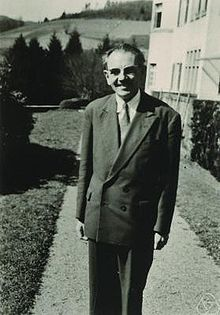
\includegraphics[height=\the\HauteurDesPhotos]{Leray}&
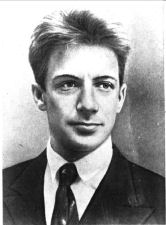
\includegraphics[height=\the\HauteurDesPhotos]{Sobolev2}\\
Leray&Sobolev%
\end{tabular}}
\ImageADroite{%
Nous arrivons maintenant à l'idée majeure de la théorie des distributions, déjà présente dans les travaux de Sobolev\index[aut]{Sobolev (Sergueï Lvovitch), 1908-1989, Russe} et Leray.\index[aut]{Leray (Jean), 1906-1998, Français} Du point de vue physique, on peut la motiver comme suit. Le résultat ou l'interprétation d'une expérience physique faisant intervenir une certaine grandeur, qui varie en fonction du temps ou de l'espace, ne dépend que très rarement des valeurs ponctuelles de cette grandeur, mais plus souvent de sa valeur moyenne (ou intégrale) prise contre une fonction du temps ou de l'espace, plus ou moins localisée. En d'autres termes, plutôt qu'une fonction $u$, c'est plutôt une «moyenne» de la forme $\int u\varphi$ qui sera accessible en pratique. Ainsi, un signal électrique oscillant avec une période très élevée fournira, de manière apparemment paradoxale, un signal plat quand on l'utilisera pour alimenter un oscilloscope: dans le processus de moyenne inhérent à la mesure, les valeurs positives et négatives se compenseront.}

Dans le cas de l'équation des ondes aussi bien que dans celui des équations de transport avec données singulières, on résout ainsi le dilemme qui nous est proposé, en reformulant l'équation par son action sur les fonctions-test.

Explicitons plus en détail la réflexion de Sobolev.\index[aut]{Sobolev (Sergueï Lvovitch), 1908-1989, Russe} Pour des raisons ayant trait
à l'analyse (fonctionnelle) de certaines classes d'équations aux dérivées partielles,
il cherchait à étudier les fonctions possédant une dérivée carré-intégrable, dans un
cadre suffisamment général... et en particulier, sans supposer la fonction dérivable!
Il montra que l'on pouvait donner une définition utile et pratique du concept de «fonction dont la dérivée est de carré intégrable», qui ne présuppose pas l'existence d'une dérivée au sens usuel. L'espace ainsi défini est aujourd'hui appelé espace de Sobolev $W^{1,2}$ ou $H^1$.

\medskip
\noindent\emph{Simplification de problèmes non linéaires ardus:}\\[+2.5mm]
L'utilisation de solutions généralisées peut venir d'une nécessité de modélisation, mais également par l'incapacité à prouver l'existence de solutions classiques. L'exemple archétypal en la matière est celui des équations de la mécanique des fluides, en particulier l'équation de Navier-Stokes\index[aut]{Navier (Claude Louis Marie Henri), 1785-1836, Français}\index[aut]{Stokes (George Gabriel), 1819-1903, Anglais} incompressible, dont la première étude mathématique moderne est due à Leray.\index[aut]{Leray (Jean), 1906-1998, Français} L'écriture même de l'équation de Navier-Stokes incompressible présuppose apparemment la dérivabilité de la fonction inconnue $u$, mais rien ne semblait permettre d'affirmer l'existence de solutions dérivables pour des données initiales assez générales. Ce problème est d'ailleurs toujours ouvert, et compte parmi les sept problèmes du millénaire de l'Institut Clay, mais nous en reparlerons au paragraphe~\ref{Sec-NavierStokes}. Leray\index[aut]{Leray (Jean), 1906-1998, Français} eut l'idée de définir une solution de l'équation de Navier-Stokes incompressible par une formulation duale qui ne présupposait pas de régularité. De telles solutions sont aujourd'hui appelées solutions faibles.

\medskip
La théorie des distributions exploite au maximum l'idée de moyenner les solutions contre des fonctions-test qui se comportent bien: on définit au départ une classe agréable de fonctions-test, à la fois très régulières et bien localisées, à savoir les fonctions indéfiniment dérivables, à support compact. Toutes les propriétés des objets que l'on cherche à définir sont alors définies en fonction des «intégrales» de ces objets contre les fonctions-test.
\end{histoire}

\medskip
\begin{definition}[Espace des fonctions tests~$\mathcal{D}(\Omega)$]
Soit~$\Omega$ un sous-espace topologique de~$\RR^n$ (ou~$\CC^n$).
\textcolorblue{L'espace des fonctions tests~$\mathcal{D}(\Omega)$} est l'ensemble des fonctions à valeurs réelles indéfiniment dérivables de~$\Omega$ à support compact inclus dans~$\Omega$.

On munit cet espace vectoriel de la topologie suivante: un ensemble~$U \subset \mathcal{D}(\Omega)$ est ouvert si et seulement si~$\forall K \subset \Omega$ compact et~$f \in U$ dont le support est inclus dans~$K$, il existe~$\epsilon > 0$ et~$k \ge 0$ tels que:
\begin{equation}
  \{ g \in \mathcal{D}(\Omega)\;\mid\; \operatorname{supp}(g) \subset K\quad\text{ et }\quad\forall x \in K,\; |f^{(k)}(x)-g^{(k)}(x)|\le \epsilon \}\;\subset\;U.
\end{equation}
Muni de cette topologie, $\mathcal{D}(\Omega)$ est un espace vectoriel topologique \textcolorred{non métrisable}.
\end{definition}

\medskip
\begin{definition}[Distribution]
\textcolorblue{Une distribution} est une \textbf{forme linéaire continue}\index{forme!linéaire} sur~$\mathcal{D}(\Omega)$.
\end{definition}

L'ensemble des distributions est donc le dual topologique de~$\mathcal{D}(\Omega)$ et est par conséquent noté~$\mathcal{D}'(\Omega)$.\index{dual topologique d'un espace vectoriel}

\begin{remarque}
L'espace des distributions est extrêmement grand, et contient tous les espaces fonctionnels que nous avons mentionnés jusqu'à présent et leur dual, y compris les espaces à poids et les espaces locaux (non présentés dans ce document).
\end{remarque}\colorgris
\begin{remarque}[Complément topologique]
L'espace~$\mathcal{D}$ n'est pas métrisable. Définir sa topologie n'est pas équivalent à définir la convergence des suites. Cependant, dans la pratique c'est presque la seule notion de convergence que l'on utilise.

\medskip
Soit~$\Omega$ un ouvert de~$\RR^n$. On muni~$\mathcal{D}'(\Omega)$ de la topologie faible-* induite par~$\mathcal{D}(\Omega)$. Alors:\\
-- $\mathcal{D}'(\Omega)$ est un espace topologique complet (et un espace de Montel);\index[aut]{Montel (Paul Antoine Aristide Montel), 1876-1975, Français}\\
-- Le dual topologique de~$\mathcal{D}'(\Omega)$ s'identifie à~$\mathcal{D}(\Omega)$, qui est donc réflexif;\\
-- La topologie de~$\mathcal{D}'(\Omega)$ n'est pas métrisable.

\medskip
Notons que la convergence dans le dual de n'importe quel espace de Sobolev implique la convergence au sens des distributions.
\end{remarque}\colorblack

Toujours aussi classiquement, si~$T$ est une distribution et~$\varphi$ une fonction test de $\mathcal{D}(\Omega)$ alors on note~$T(\varphi)=\langle T,\varphi \rangle$. (où~$\langle\cdot,\cdot\rangle$ désigne comme d'habitude le crochet de dualité).
\medskipvm
Dans~$\mathcal{D}'(\mathbb{R})$, l'application qui à~$\varphi$ associe~$\varphi(0)$ est une distribution et c'est la distribution de Dirac\index{distribution!de Dirac}\index[aut]{Dirac (Paul Adrien Maurice), 1902-1984, Anglais}:
\begin{equation}
\langle\delta,\varphi\rangle=\varphi(0)
\end{equation}
\medskipvm
Une propriété fondamentales est que \textcolorblue{toute fonction localement intégrable~$f$ représente aussi une distribution~$T_f$ définie par la forme intégrale suivante}:
\begin{equation}
  \langle T_f,\varphi\rangle=\int_{\mathbb{R}}f(x)\varphi(x)\,\dd x, \quad \forall \varphi\in\mathcal{D}(\Omega)
\end{equation}

\medskip
\begin{remarque}[Commentaire sur le choix de l'espace~$\mathcal{D}$]\colorgreen
Pourquoi ce choix, qui semble assez restrictif?
Notons tout d'abord que plus on restreint la classe des fonctions-tests, plus l'espace des distributions définies sur ces fonctions sera grand. De plus, le fait que les fonctions-tests soient de classe~$C^\infty$ n'est pas très restrictif en fait, car toute fonction continue à support borné est limite uniforme de telles fonctions. Le fait qu'elles soient de support borné est levé si l'on considère l'espace de Schwartz~$\mathcal{S}$ des fonctions-tests lisses, i.e. de classe~$C^\infty$, et à décroissance rapide ainsi que toutes leurs dérivées. Dans ce cas, l'espace dual~$\mathcal{S}'$ qui en résulte est plus petit que~$\mathcal{D}$. Pour plus de détails sur ce sujet, on consultera un cours sur la transformée de Fourier, par exemple un cours de traitement du signal.
\end{remarque}

\medskip
\section{Dérivées au sens des distributions}\index{dérivée!au sens des distributions}
Pour définir la dérivée d'une distribution, considérons d'abord le cas d'une fonction différentiable et intégrable~$f:\mathbb{R}\rightarrow\mathbb{R}$.
Soit~$\varphi$ une fonction test, supposée régulière et à support compact.
Une intégration par parties permet d'écrire:
\begin{equation}
  \int_\RR f'(x) \varphi(x)\,\dd x = -\int_\RR f(x)\varphi'(x)\,\dd x \qquad\text{ soit }\qquad I_{f'}(\varphi)=I_{-f}(\varphi')
\end{equation}
En effet, puisque la fonction~$\varphi$ est nulle en dehors d'un ensemble borné (elle est à support compact), les termes de bords s'annulent.

\medskip
\begin{definition}[Dérivée d'une distribution]\label{Def-DerivDistrib}
Si~$S$ est une distribution, cet exemple suggère que l'on puisse \textcolorblue{définir sa dérivée~$S'$ comme la forme linéaire} qui à une fonction test~$\varphi$ fait correspondre la valeur~$- S(\varphi')$. On pose donc:
\begin{equation}\colorred
  \langle S', \varphi \rangle = - \langle S, \varphi' \rangle
\end{equation}
Cette définition étend la notion classique de dérivée: chaque distribution devient \textcolorred{indéfiniment dérivable} et l'on peut montrer les propriétés usuelles des dérivées.
\end{definition}

\medskip
Cette notion peut aussi se définir comme la dérivée du produit de dualité~$\langle S,\varphi\rangle$.
On note~$\varphi_h:x\rightarrow\varphi(x-h)$ la translatée de~$\varphi$ par la valeur~$h\in{\mathbb R}$, alors, en utilisant la linéarité et la continuité par rapport au deuxième terme:
\begin{equation}
\langle\frac{\dd S}{\dd x},\varphi\rangle= \lim_{h\rightarrow 0}\frac{ \langle S,\varphi_h\rangle- \langle S,\varphi\rangle}{h}
= \langle S,\lim_{h\rightarrow 0} \frac{\varphi_h-\varphi}{h} \rangle= -\langle S,\frac{\dd\varphi}{\dd x}\rangle
\end{equation}
Lorsque la distribution~$S$ modélise un phénomène physique, la fonction test~$\varphi$ peut s'interpréter comme un instrument de mesure, $\langle S,\varphi\rangle$ en étant le résultat; la définition ci-dessus représente alors la mesure expérimentale (au moins de pensée) de la dérivée du phénomène~$S$ à l'aide de l'instrument~$\varphi$.

\medskip
\textcolorgris{Nous définirons dans un autre cours (sur le traitement du signal) les notions de distribution à support compact, les distributions tempérées et la décroissance rapide utiles en analyse de Fourier ainsi que les espaces de Schwartz.}

\colorblack
\begin{remarque}[Complément au sujet des opérations sur des distributions]\colorgris
L'addition, la soustraction et la multiplication par un scalaire sont telles qu'on les imagine.

Le cas de la dérivation (pour lequel les distributions ont été inventées) a été traité ci-dessus à la définition~\ref{Def-DerivDistrib}.

\medskip
Les distributions permettent de changer momentanément l'ouvert~$\Omega$ sur lequel on travaille. Pour cela, on dispose des trois opérations suivantes:\\
-- Opération de \emph{restriction}:
Soient~$\Omega$ un ouvert de~$\RR^n$, et~$\Omega'$ un ouvert de~$\Omega$. Toute distribution~$T\in\mathcal{D}'(\Omega)$ définit une distribution sur~$\Omega'$, simplement par restriction de l'espace des fonctions test: $\mathcal{D}(\Omega') \subset \mathcal{D}(\Omega)$. On peut donc restreindre une distribution à un ouvert plus petit que celui sur lequel elle était définie initialement.\\
-- Opération de \emph{localisation}: Soient un compact~$K$ (au voisinage duquel on veut étudier la distribution), $O$ un ouvert contenant~$K$, et~$T\in\mathcal{D}(\Omega)$ une distribution. On peut trouver une autre distribution~$T'$ dont le support est inclus dans~$O$, et qui coïncide avec~$T$ dans un voisinage de~$K$. Pour cela il suffit de définir $\langle T',\varphi\rangle = \langle T,\chi_\varphi\rangle$ où $\chi_\varphi$ est une fonction plateau identiquement 1 au voisinage de~$K$,à support compact inclus dans~$O$.\\
-- Opération de \emph{recollement}: Soient~$(\Omega_i)_{i\in J}$ une famille(éventuellement
infinie) d'ouverts de~$\RR^n$, et~$\Omega$ la réunion des~$\Omega_i$. Pour chaque~$i$, on se donne une distribution~$T_i\in\mathcal{D}'(\Omega_i)$. On peut définir dans~$\Omega$ une distribution~$T$ dont la restriction à chaque~$\Omega_i$ soit~$T_i$, sous la condition nécessaire que~$T_i=T_j$ dans~$\Omega_i\cap\Omega_j$. On utilise le théorème de partition de l'unité pour construire cette distribution, et on montre que celle-ci est indépendante de la partition choisie.

\medskip
La multiplication des distributions pose des problèmes considérables et ne se résout que partiellement.
\end{remarque}

\begin{remarque}[Exemples de calculs avec les distributions]\colorgris
Considérons la fonction~$f(x) =|x|$ sur~$\RR$. Alors~$f'$ est la fonction «signe», $f'' = 2\delta_0$, $f'''$ vaut 2 fois l'application «évaluation de la dérivée en 0». Attention donc à ne pas confondre ces dérivées au sens des distributions avec les dérivées presque partout, qui sont nulles à partir du rang 2.

\medskip
Soit~$f(x)=x\log|x|-x$ dans~$\RR$, alors on peut écrire, au sens des distributions, $f'(x) = \log|x|$, $f''(x) = v.p.(1/x)$ (où $v.p.$ est la valeur principale).

\medskip
Soit~$(u_n)$ la suite de fonctions définie par~$u_n(x) = (1/n)sin(nx)$. Alors la famille $(u'_n)$ converge au sens des distributions vers 0.
\end{remarque}
\colorblack


\medskip
\section{Espaces~$W^{m,p}(\Omega)$}\index{espace!de Sobolev!$W^{m,p}(\Omega)$}\index[aut]{Sobolev (Sergueï Lvovitch), 1908-1989, Russe}

\begin{definition}[Espace~$W^{m,p}(\Omega)$]
Soient~$\Omega \subset \RR^n$ un ouvert quelconque, $p$ un réel tel que~$1\leqslant p\leqslant \infty$ et~$m$ un entier naturel positif.
On définit l'espace de Sobolev~$W^{m,p}(\Omega)$ par:
\begin{equation}\label{Eq-SoboW}\colorred
W^{m, p}(\Omega)=\{u\in L^p(\Omega); D^\alpha u \in L^p(\Omega)\}
\end{equation}
où~$\alpha$ est un multi-indice tel que~$0\leqslant |\alpha| \leqslant m$ , $D^\alpha u$ est une dérivée partielle de~$u$ au sens faible (i.e. au sens des distributions) et~$L^p$ un espace de Lebesgue.
\end{definition}

\medskip
La norme sur~$W^{m,p}(\Omega)$ est:\index{norme!sur~$W^{m,p}(\Omega)$}
\begin{equation}
\| u \|_{W^{m, p}} = \begin{cases} \left( \sum \limits_{0\leqslant | \alpha | \leqslant m} \| D^{\alpha} u \|_{L^{p}}^{p} \right)^{1/p}, & 1 \leqslant p < + \infty; \\ \max\limits _{0\leqslant | \alpha | \leqslant m} \| D^{\alpha} u \|_{L^{\infty}}, & p = + \infty; \end{cases}
\end{equation}
où~$\|\cdot\|_{L^{p}}$ désigne la norme des espaces de Lebesgue.
Muni de cette norme~$W^{m,p}(\Omega)$ est un espace de Banach.\index{espace!de Banach}
Dans le cas où~$p<\infty$, c'est aussi un espace séparable.
\medskipvm
La norme:
\begin{equation}
\| u \|_{W^{m, p}} = 
   \begin{cases} 
   \sum\limits _{0\leqslant | \alpha | \leqslant m} \| D^{\alpha} u \|_{L^{p}}, & 1 \leqslant p < + \infty; \\ \sum\limits _{0 \leqslant | \alpha | \leqslant m} \| D^{\alpha} u \|_{L^{\infty}}, & p = + \infty. 
   \end{cases}
\end{equation}
est une norme équivalente à la précédente. On utilisera donc indifféremment l'une de ces normes, et on notera la norme employée~$\|\cdot\|_{W^{m, p}}$ ou plutôt~$\|\cdot\|_{m, p}$.

\medskip\colorgris
Si~$p<\infty$, alors~$W^{m,p}(\Omega)$ est identique à la fermeture de l'ensemble $\lbrace u \in C^m(\Omega) ; \left\|u \right\|_{m,p} < \infty \rbrace$ par rapport à la norme $\left\|\cdot\right\|_{m,p}$ où~$C^m(\Omega)$ désigne l'espace de Hölder des fonctions de
classe~$m$ sur~$\Omega$.
\medskipvm
\begin{remarque}
Le théorème de Meyers-Serrin\index{théorème!de Meyers-Serrin}\index[aut]{Meyers (Norman George), 1930-, Américain}\index[aut]{Serrin (James Burton), 1926-2012, Américain} dit~«$H=W$» (qui est le titre de leur article de 1964 \cite{bib-WH}) montre l'équivalence de deux définitions des espaces de Sobolev~$W^{m,p}(\Omega) = H^{m,p}(\Omega)$, i.e. dans notre cas, donne une définition équivalente, par complétion de l'espace vectoriel normé:
\begin{equation}
\{u\in C^\infty(\Omega);\| u \|_{H^{m, p}} < \infty\}\quad\text{ avec }\quad
\| u \|_{H^{m, p}}:= \left( \sum_{| \alpha | \leqslant m} \| D^{\alpha} u \|_{L^{p}}^p \right)^{1/p}
\end{equation}
où~$D^\alpha u$ est une dérivée partielle de~$u$ au sens classique ($u \in C^\infty(\Omega)$).
\end{remarque}
\colorblack


\medskip
\section{Espaces~$H^m(\Omega)$, $H^m_0(\Omega)$ et~$H^{-m}(\Omega)$}\index{espace!de Sobolev!$H^m(\Omega)$}\index[aut]{Sobolev (Sergueï Lvovitch), 1908-1989, Russe}\index{espace!de Sobolev!$H_0^m(\Omega$}\index{espace!de Sobolev!$H^{-m}(\Omega)$}

\begin{definition}[Espace~$H^m(\Omega)$]\label{Th-Hm}\index{espace!de Sobolev!$H^m(\Omega)$}
\textcolorblue{Dans le cas~$p=2$, on note~$H^m(\Omega)$ l'espace~$W^{m,2}(\Omega)$, défini par la relation (\ref{Eq-SoboW}).}
\end{definition}

\medskip
Les espaces de Sobolev~$H^m$ ont un intérêt particulier car il s'agit alors d'\textcolorred{espaces de Hilbert.}\index{espace!de Hilbert}\index[aut]{Hilbert (David), 1862-1943, Allemand}
Leur norme est induite par le produit intérieur suivant:\index{produit scalaire!de~$H^m(\Omega)$}
\begin{equation}(u,v)_{m} =\sum \limits _{0 \leqslant \vert \alpha\vert\leqslant m} \left( D^{\alpha} u, D^{\alpha} v\right)
\end{equation}
où: 
\begin{equation}(u,v) = \int_{\Omega} u(x) \overline{v}(x)\, \dd x
\end{equation}
est le produit intérieur dans $L^{2} ( \Omega)$; produit scalaire dans le cas réel, hermitien\index[aut]{Hermite (Charles), 1822-1901, Français} dans le cas complexe.

%\medskip
\begin{theoreme}
Si~$\Omega$ est Lipschitzien, alors l'ensemble~$C^\infty(\overline{\Omega})$ des fonctions régulières jusqu'au bord de~$\Omega$ est dense dans~$H^m(\Omega)$.
\end{theoreme}

\colorgris
\begin{remarque}[Complément]
De plus, dans le cas où la transformation de Fourier peut être définie dans~$L^{2} ( \Omega)$, l'espace~$H^k(\Omega)$ peut être défini de façon naturelle à partir de la transformée de Fourier (voir cours sur le traitement du signal).
\medskipvm
Par exemple si~$\Omega = \RR^{n}$, si~$\widehat{u}$ est la transformée de Fourier de~$u$:
\begin{equation}
H^{m}\left( \RR ^{n}\right)=\lbrace u \in L^{2}\left( \RR^{n}\right);\; \int_{\RR^{n}}\vert\hat{u}\left( \xi\right) \xi^{\alpha}\vert ^{2}\dd\xi \;<\infty
\end{equation}
pour $\vert\alpha\vert \leqslant m \rbrace$, ou ce qui est équivalent:
\begin{equation}
H^{m}\left( \RR ^{n}\right)=\left\lbrace u \in L^{2}\left( \RR^{n}\right);\; \int_{\RR^{n}}\vert\hat{u}\left( \xi\right) \vert ^{2}\left( 1+\xi^{2}\right)^{m} \dd\xi \;<\infty \right\rbrace
\end{equation}
et que:
\begin{equation}
(u,v)_{m}=\int_{\RR^{n}}\hat{u}(\xi) \overline{\hat{v}(\xi)} \left(1 + \xi^{2} \right) ^{m} \dd\xi
\end{equation}
est un produit hermitien\index[aut]{Hermite (Charles), 1822-1901, Français} équivalent à celui défini plus haut. Encore, si~$\Omega =\intoo{0}{1}$, on vérifie que:
\begin{equation}
H^m(\intoo{0}{1}) = \left\{ u\in L^2(\intoo{0}{1});\sum\limits_{n=-\infty}^{+\infty} (1+n^2 + n^4 + \dotsb + n^{2m}) |\widehat{u}_n|^2 < \infty \right\}
\end{equation}
où~$\widehat{u}_n$ est la série de Fourier de~$u$.
On peut aussi utiliser la norme équivalente:
\begin{equation}
\|u\|^2=\sum\limits_{n=-\infty}^{+\infty} (1 + |n|^{2})^m |\widehat{u}_n|^2
\end{equation}
\end{remarque}
\colorblack


\medskip
%\section{Espaces~$H^m_0(\Omega)$}\index{espace!de Sobolev!$H_0^m(\Omega$}\index[aut]{Sobolev (Sergueï Lvovitch), 1908-1989, Russe}

\begin{definition}[Espace~$H^m_0(\Omega)$]\label{Th-Hmz}\index{espace!de Sobolev!$H_0^m(\Omega$}
On définit \textcolorblue{$H^m_0(\Omega)$} comme l'adhérence dans~$H^m(\Omega)$ de~$\mathcal{D}(\Omega)$, ensemble des fonctions de classe~$C^\infty$ et à support compact dans~$\Omega$.
\end{definition}
Plus exactement et de manière générale, $W^{m,p}_0$ est l'adhérence de~$\mathcal{D}(\Omega)$ dans l'espace $W^{m,p}$. La définition ci-dessus correspond donc au cas~$p=2$.

\medskip
\begin{remarque}
Il faut bien comprendre que cela signifie quelque chose de simple: c'est l'ensemble constitué des fonctions qui sont à la fois~$\mathcal{D}(\Omega)$ et~$H^m(\Omega)$.
Comme on s'intéresse à la frontière (puisque l'on prend l'adhérence), et que~$\Omega$ est un ouvert, la valeur que prennent les fonctions de cet ensemble sur la frontière est celle que prennent les fonctions de classe~$C^\infty$ et à support compact dans~$\Omega$, soit~$0$ !
\end{remarque}

\textcolorgreen{Ainsi, «physiquement» les espaces~$H^m_0(\Omega)$ sont les fonctions de~$H^m(\Omega)$ qui sont nulles sur~$\Gamma=\partial\Omega$, ainsi que leurs dérivées «normales» jusqu'à l'ordre~$m-1$.}\index{dérivée!normale}
Plus mathématiquement, on dit que ces fonctions sont de trace nulle sur la frontière, comme par exemple:
\begin{equation}
  H_0^2(\Omega)=\left\{v / v\in H^2(\Omega), v|_\Gamma=0,
  \frac{\partial v}{\partial n}|_\Gamma=0\right\}
\end{equation}
Les espaces trace sont définis plus loin.\index{espace!trace}.
\medskipvm
\textcolorred{Les espaces~$H^m_0(\Omega)$ sont des espaces de Hilbert.}\index{espace!de Hilbert}\index[aut]{Hilbert (David), 1862-1943, Allemand}


\medskip
%\section{Espaces~$H^{-m}(\Omega)$}\index{espace!de Sobolev!$H^{-m}(\Omega)$}\index[aut]{Sobolev (Sergueï Lvovitch), 1908-1989, Russe}
%\colorgris
\begin{definition}[Espace~$H^{-m}(\Omega)$]\label{Th-Hmm}\index{espace!de Sobolev!$H^{-m}(\Omega)$}
Il est possible de caractériser le dual topologique de~$H^m_0(\Omega)$ de la façon suivante.\index{espace!vectoriel!topologique} Pour tout~$m\ge 1$, on définit l'espace des distributions suivant:
\begin{equation}
H^{-m}(\Omega) =\left\{
f\in \mathcal{D}'(\Omega), f=\dsum_{|\alpha|\le m} \partial^\alpha f_\alpha,
\text{ avec } f_\alpha\in L^2(\Omega)
\right\}
\end{equation}
muni de la norme:\index{norme!sur~$H^{-m}(\Omega)$}
\begin{equation}
\|f\|_{H^{-m}} = \inf \left( \dsum_{|\alpha|\le m} \|f_\alpha\|^2_{L^2} \right)^{1\over2}
\end{equation}
l'infimum étant pris sur toutes les décompositions possibles de~$f$ sous la forme intervenant dans la définition de~$H^{-m}$.
\end{definition}
\medskipvm
Ainsi défini, l'espace~$H^{-m}(\Omega)$ est un espace de Hilbert isomorphe au dual topologique de~$H^m_0(\Omega)$, et le crochet de dualité s'écrit:\index{dual topologique d'un espace vectoriel}
\begin{equation}
\langle f,u\rangle_{H^{-m},H_0^m} = \dsum_{|\alpha\le m} (-1)^\alpha \dint_\Omega
f_\alpha \partial^\alpha u \dd x,
\quad \forall f\in H^{-m}(\Omega),\quad \forall u\in H^m_0(\Omega)
\end{equation}
Cette formule ne dépend pas de la décomposition de~$f$ en somme des~$\partial^\alpha f_\alpha$.
\medskipvm
Remarquons que le dual de~$H^m(\Omega)$ n'est pas un espace de distribution et ne possède donc pas de caractérisation aussi simple.
%\colorblack

\medskip
\section{Prise en compte du contour du domaine}

\subsection{Trace}\label{Sec-SoboTrace}\index{espace!trace}
Dans ce paragraphe, nous essayons de présenter la notion de trace de manière simple et intuitive.

\medskip
\textcolorgreen{Afin de pouvoir parler de la valeur d'une fonction sur la frontière de~$\Omega$, il nous faut définir le prolongement (la trace) d'une fonction sur ce bord.}

\medskip
Cas~$n=1$:
on considère un intervalle ouvert~$I =]a;b[$ borné. On a vu que~$H^1(I)\subset C^0(\overline{I})$.
Donc, pour~$u\in H^1(I)$, $u$ est continue sur~$[a;b]$, et~$u(a)$ et~$u(b)$ sont bien définies.

\medskip
Cas~$n>1$:
il nous faut définir la trace lorsque l'on n'a plus~$H^1(I)\subset C^0(\overline{I})$. On procède ainsi:
\begin{itemize}
  \item On définit l'espace:
	\begin{equation}C^1(\overline{\Omega}) = \left\{\varphi:\Omega\rightarrow\RR/ \exists O
	\text{ ouvert contenant } \overline{\Omega}, \exists \psi\in C^1(O), \psi_{|\Omega}=\varphi
	\right\}\end{equation}
	$C^1(\overline{\Omega})$ est donc l'espace des fonctions~$C^1$ sur~$\Omega$, prolongeables par continuité sur~$\partial\Omega$ et dont le gradient est lui-aussi prolongeable par continuité.
	Il n'y a donc pas de problème pour définir la trace de telles fonctions.
  \item On montre que, si~$\Omega$ est un ouvert borné de frontière~$\partial\Omega$  «assez régulière», alors~$C^1(\overline{\Omega})$ est dense dans~$H^1(\Omega)$.
  \item L'application linéaire continue, qui à toute fonction~$u$ de~$C^1(\overline{\Omega})$ associe sa trace sur~$\partial\Omega$, se prolonge alors en une application linéaire continue de~$H^1(\Omega)$ dans~$L^2(\partial\Omega)$, notée~$\gamma_0$, qu'on appelle \textcolorblue{application trace}. On dit que~$\gamma_0(u)$ est la trace de~$u$ sur $\partial\Omega$.
\end{itemize}
Pour une fonction~$u$ de~$H^1(\Omega)$ qui soit en même temps continue sur~$\overline{\Omega}$, on a évidemment~$\gamma_0(u) = u_{|\partial\Omega}$. \textcolorred{C'est pourquoi on note souvent par abus simplement~$u_{|\partial\Omega}$ plutôt que~$\gamma_0(u)$.}

\medskip
De manière analogue, on peut définir~$\gamma_1$, l'application trace qui permet de prolonger la définition usuelle de la dérivée normale sur~$\partial\Omega$.
Pour~$u\in H^2(\Omega)$, on a~$\partial_iu\in H^1(\Omega)$, $\forall i=1,\ldots,n$ et on peut donc définir~$\gamma_0(\partial_iu)$. La frontière~$\partial\Omega$ étant «assez régulière» (par exemple, idéalement, de classe~$C^1$), on peut définir la normale~$n = (n_1,\ldots,n_n)^T$ en tout point de~$\partial\Omega$.
On pose alors:
\begin{equation}\gamma_1(u) = \dsum_{i=1}^n \gamma_0(\partial_iu)n_i\end{equation}
Cette application continue~$\gamma_1$ de~$H^2(\Omega)$ dans~$L^2(\partial\Omega)$) permet donc bien de prolonger la définition usuelle de la dérivée normale.
Dans le cas où~$u$ est une fonction de~$H^2(\Omega)$ qui soit en même temps dans~$C^1(\overline{\Omega})$, la dérivée normale au sens usuel de~$u$ existe, et~$\gamma_1(u)$ lui est évidemment égale.
\textcolorred{C'est pourquoi on note souvent, par abus, $\partial_n u$ plutôt que~$\gamma_1(u)$.}

\medskip
\subsection{Espace trace}\index{espace!trace}\index[aut]{Sobolev (Sergueï Lvovitch), 1908-1989, Russe}

%\textcolorgreen{Compte tenu du paragraphe précédent qui exposait la notion de trace, cette section n'a plus vraiment d'intérêt si l'on ne souhaite pas entrer trop dans les détails mathématiques.}
%
%\medskip
Dans le cas d'exposant entier, on note souvent l'ordre avec la lettre~$m$, dans le cas non-entier, on utilisera la lettre~$s$, et donc les espaces seront notés:~$W^{s,p}$ ou~$H^s$.

\medskip
\subsubsection{Cas~$p=2$ et~$\Omega=\RR^{n}$}

\colorgris
Dans ce cas, l'espace de Sobolev~$H^{s}(\RR^n)$, $s\geqslant 0$, peut être défini grâce à la transformée de Fourier:
\begin{equation}
H^{s} (\RR^n) = \left\{ u \in L^{2}(\RR^n) \colon \int_{\RR^n} ( 1 + | \xi |^{2} )^{s} | \hat{u} (\xi) |^{2} \, \dd\xi < + \infty \right\}.
\end{equation}
$H^{s}(\RR^n)$ est un espace de Hilbert muni de la norme:
\begin{equation}\| u \|_{H^{s}}^{2} = \int_{\RR^n} ( 1 + | \xi |^{2} )^{s} | \hat{u} (\xi) |^{2} \, \dd\xi \end{equation}
\colorblack

\medskip
\subsubsection{Cas~$p=2$ et~$\Omega \subset \RR^{n}$ quelconque}
On peut alors caractériser les espaces de Sobolev d'ordre fractionnaire~$H^s(\Omega)$ grâce au produit intérieur donné par:
\begin{equation}
(u, v)_{H^{s} (\Omega)} = (u,v)_{H^{k} (\Omega)} + \sum_{| \alpha | = k} \int_{\Omega} \int_{\Omega} \frac{( D^{\alpha}u (x) - D^{\alpha}u (y) ) (D^{\alpha}v (x) - D^{\alpha}v (y) )}{| x - y |^{n + 2 t}} \, \dd x \dd y
\end{equation}
où~$s = k + T$, $k$ est un entier tel que~$0 < T < 1$ et~$n$ est la dimension du domaine $\Omega \subset \RR^{n}$.
La norme induite est essentiellement l'analogue pour~$L^2$ de la continuité au sens de Hölder.

\medskip
\subsubsection{Cas~$p\neq 2$ et~$\Omega = \intoo{0}{1}$}

\colorgris
On définit un opérateur~$D^s$ de dérivation d'ordre fractionnaire~$s$ par:
\begin{equation}
D^{s}u=\sum_{n=-\infty}^\infty (in)^s\widehat{u}(n)\mathrm{e}^{int}
\end{equation}

En d'autres mots, il s'agit de prendre la transformée de Fourier, de la multiplier par~$(in)^s$ et à prendre la transformée de Fourier inverse (les opérateurs définis par la séquence: transformation de Fourier --- multiplication --- transformation inverse de Fourier sont appelés des multiplicateurs de Fourier).
Cet opérateur permet de définir la norme de Sobolev de~$H^s(\intoo{0}{1})$ par: 
$\|u\|_{s,p}=\|u\|_p+\|D^s u\|_p$ et de définir l'espace de Sobolev~$H^s(\intoo{0}{1})$
comme l'espace des fonctions pour lesquelles cette norme est finie.
\colorblack

\medskip
\subsubsection{Cas général des espaces~$H^s$}\index[aut]{Sobolev (Sergueï Lvovitch), 1908-1989, Russe}

Soit~$s > \frac{1}{2}$. Si~$\Omega$ est un ouvert dont la frontière~$\partial \Omega$ est «suffisamment régulière», alors on peut définir un \textcolorblue{opérateur de trace~$T$} qui à une fonction~$u \in H^{s}(\Omega)$ lui associe sa trace, i.e sa restriction sur la frontière de~$\Omega$: \textcolorgreen{$Tu=u|_{\partial \Omega}$.}

Une hypothèse simple qui satisfasse la condition de régularité est que~$\partial \Omega$ soit uniformément~$C^m$ pour~$m \geqslant s$.
Ainsi défini, cet opérateur de trace~$T$ a pour domaine de définition~$H^s(\Omega)$ et son image est précisément~$H^{s-1/2}(\partial \Omega)$.

En fait, $T$ est d'abord défini pour les fonctions indéfiniment dérivables et cette définition est ensuite étendue par continuité à tout l'ensemble~$H^s(\Omega)$.
De façon intuitive, on peut dire que l'on perd en régularité «une demi-dérivée» en prenant la trace d'une fonction de~$H^s(\Omega)$.

\textcolorgreen{Nous nous servirons de ces espaces dans le cas des éléments finis pour un problème de continuité des contraintes à une interface entre deux milieux solides ayant des propriété matérielles différentes. Ce problème sera abordé plusieurs fois dans ce document, et le paragraphe~\ref{Sec-interf} fera une synthèse des stratégies possibles pour le résoudre.}

\medskip
\subsubsection{Cas général des espaces~$W^{s,p}$}\index[aut]{Sobolev (Sergueï Lvovitch), 1908-1989, Russe}

\colorgris
Définir la trace d'une fonction de~$W^{s,p}$ est très difficile et demande d'utiliser les techniques plus compliqués (dont les espaces de Besov).

De façon plus intuitive, on peut dire que l'on perd en régularité~$1/p$-ème de dérivée en prenant la trace d'une fonction de~$W^{s,p}(\Omega)$.
\colorblack



\medskip
\section{Espaces~$H^1(\Omega)$, $H^1_0(\Omega)$ et~$H^{-1}(\Omega)$}\index{espace!de Sobolev!$H_0^1(\Omega)$}\index{espace!de Sobolev!$H^1(\Omega)$}\index{espace!de Sobolev!$H^{-1}(\Omega)$}\index[aut]{Sobolev (Sergueï Lvovitch), 1908-1989, Russe}

Nous avons déjà défini les espaces~$H^m(\Omega)$, $H^m_0(\Omega)$ et~$H^{-m}(\Omega)$.
Toutefois, dans la pratique, nous n'irons guerre au delà de $m=2$, et même le plus souvent nous nous contenterons de $m=1$. Nous donnons ici quelques compléments dans ce dernier cas.

\medskip
En application de la définition~\ref{Th-Hm}, nous avons:
\begin{equation}
H^1(\Omega)=\left\lbrace u\in L^2(\Omega);\; \forall i =1,\ldots,n,\; \frac{\partial u}{\partial x_i}\in L^2(\Omega) \right\rbrace
\end{equation}
Muni du produit scalaire:
\begin{equation}(u,v)_1 = \dint_{\Omega} \left(uv + \sum_{i=1}^N \frac{\partial u}{\partial x_i} \frac{\partial v}{\partial x_i} \right )
\end{equation}
$H^1(\Omega)$ est un espace de Hilbert.\index{produit scalaire!de~$H^1(\Omega)$}\index{espace!de Hilbert}\index[aut]{Hilbert (David), 1862-1943, Allemand}

\textcolorgreen{%
En physique et en mécanique, l'espace~$H^1(\Omega)$ est également appelé «espace d'énergie» au sens où il est constitué des fonctions d'énergie finie (i.e. de norme finie).}\index{espace!d'énergie}


\medskip
\begin{theoreme}[Théorème de densité]\index{théorème!de densité}
Si~$\Omega$ est un borné régulier de classe~$C^1$, ou si~$\Omega=\RR^n_+$, ou encore si $\Omega=\RR^n$, alors~$C_c^\infty(\overline{\Omega})$ est dense dans~$H^1(\Omega)$.
\end{theoreme}

\textcolorgreen{%
En pratique, il est très important de savoir si les fonctions régulières sont denses dans l'espace de Sobolev~$H^1(\Omega)$. Cela justifie en partie la notion d'espace de Sobolev qui apparaît ainsi très simplement comme l'ensemble des fonctions régulières complétées par les limites des suites de fonctions régulières dans la norme de l'énergie.
Cela permet de démontrer facilement de nombreuses propriétés en les établissant d'abord sur les fonctions régulières puis en utilisant un argument de densité.}

\medskip
Par définition de~$H_{0}^1(\Omega)$, et en prenant en compte une remarque précédente:
\begin{equation}
  H_0^1(\Omega)=\left\{v\left/v\in H^1(\Omega), v|_\Gamma=0\right.\right\}
\end{equation}
\textcolorgreen{On voit que sur cet espace, la condition de Dirichlet est satisfaite automatiquement sur tout le pourtour~$\Gamma=\partial\Omega$.}\index{condition aux limites!de Dirichlet}\index[aut]{Dirichlet (Johann Peter Gustav Lejeune), 1805-1859, Allemand}
\medskipvm
La frontière~$\Gamma$ est généralement partitionnée en deux sous-frontière $\Gamma_D$ et~$\Gamma_N$ sur lesquelles on satisfait les conditions de Dirichlet et de Neumann respectivement~:~$\Gamma=\Gamma_D \cup \Gamma_N$\index[aut]{Neumann (Carl Gottfried), 1832-1925, Allemand}\index{condition aux limites!de Neumann}
\begin{equation}
  H_{0,D}^1(\Omega)=\left\{v\left/v\in H^1(\Omega), v|_{\Gamma_D}=0\right.\right\}
\end{equation}
et \textcolorred{$H_0^1(\Omega)\subset H_{0,D}^1(\Omega)\subset H^1(\Omega)$.}

\medskip
\textcolorgris{%
On rappelle que l'espace~$H^{-1}(\Omega)$ est le dual de~$H^1_0(\Omega)$.
Or, grâce au théorème de représentation de Riesz-Fréchet (théorème \ref{Th-RF} du chapitre~\ref{Ch_FFaible} portant sur les formulations faibles), on sait que l'on peut identifier le dual d'un espace de Hilbert avec lui-même.
Cependant en pratique, on n'identifie pas~$H^{-1}(\Omega)$ et~$H^1_0(\Omega)$.
En effet, ayant défini~$H^1_0(\Omega)$ comme un sous-espace strict mais dense de~$L^2(\Omega)$, et ayant déjà identifié~$L^2(\Omega)$ à son dual (muni du produit scalaire usuel, voir chapitre précédent), on ne peut pas en plus identifier~$H^{-1}(\Omega)$ et~$H^1_0(\Omega)$ (avec un autre produit scalaire). On a donc les inclusions strictes suivantes:
\begin{equation} H^1_0(\Omega)\subset L^2(\Omega)\equiv \left(L^2(\Omega)\right)'\subset H^{-1}(\Omega)
\end{equation}}
\medskipvm
\textcolormagenta{%
Grâce à~$H^{-1}(\Omega)$, on pourrait définir une nouvelle notion de dérivation pour les fonctions de~$L^2(\Omega)$, plus faible encore que la dérivée faible.
Devant l'afflux de notions de dérivations, rassurons le lecteur en disant qu'elles sont toutes des avatars de la dérivation au sens des distributions (c'est l'intérêt de la théorie des distribution que d'avoir unifié ces divers types de dérivation).}

\bigskip
L'exemple le plus simple à retenir, et le plus utile pour la suite, est que tout élément~$f$ de~$H^{-1}(\Omega)$ s'écrit, au sens des distributions, sous la forme:
\begin{equation}\colorred
f = u + \dive G
\end{equation}
avec~$u \in L^2(\Omega)$ et~$G \in (L^2(\Omega))^n$.
\medskip
\begin{theoreme}[Dérivation des fonctions composées dans les espaces de Sobolev]\index{théorème!de dérivation des fonctions composées dans les espaces de Sobolev}
%\colorgris
Soit~$\Omega$ un ouvert borné de~$\RR^n$.
Pour toute fonction~$u \in H^1(\Omega)$ et toute fonction~$T: \RR \to \RR$ de classe $C^1$ à dérivée bornée nous avons:
\begin{equation}
T(u) \in H^1(\Omega)\quad\text{ et }\quad\nabla T(u) = T'(u)\nabla u
\end{equation}
De plus, l'application~$u \in H^1(\Omega) \mapsto T(u) \in H^1(\Omega)$ est continue.
\end{theoreme}
\colorblack
\medskip
On se contente ici de donner les résultats concernant l'espace~$H^1(\Omega)$ même si des résultats similaires peuvent êtres démontrés pour les espaces~$H^m(\Omega)$ ou les espaces~$W^{1,p}(\Omega)$, avec~$p\ne 2$ (voir théorème~\ref{Th-Inj-Sobo}).
Soit~$\Omega$ un ouvert borné Lipschitzien de~$\RR^n$.
\begin{itemize}
  \item si~$n=1$, on a une injection continue de~$H^1(\Omega)$ dans l'espace de Hölder~$C^{0,\frac12}(\Omega)$;
  \item si~$n=2$, on a une injection continue de~$H^1(\Omega)$ dans l'espace $L^p(\Omega)$ pour tout~$p<\infty$ (et donc pas dans~$L^\infty(\Omega)$.
  \item si~$n\ge 3$, on a une injection continue de~$H^1(\Omega)$ dans l'espace $L^{p*}(\Omega)$ avec~$p*=\frac{2n}{n-2}$.
\end{itemize}
De plus les injection non critiques sont compactes.

Comme on va s'intéresser par la suite à la discrétisation de problème aux dérivées partielles, le cadre de domaines bornés nous suffira.

%\medskip
%\section{Relèvement d'espace}
\medskip%\ifVersionDuDocEstVincent\else\newpage\fi
\section{Espaces~$H(\dive)$ et~$H(\rot)$}\index[aut]{Sobolev (Sergueï Lvovitch), 1908-1989, Russe}

\begin{definition}[Espace~$H(\dive,\Omega)$]\index{espace!de Sobolev!$H(\dive)$}
L'espace \textcolorblue{$H(\dive,\Omega)$} est un espace intermédiaire entre~$L^2(\Omega)$ et $H^1(\Omega)$, qui est défini par:
\begin{equation}
H(\dive,\Omega)=\left\{ f\in L^2(\Omega)^n;\; \dive f\in L^2(\Omega)\right\}
\end{equation}
%où~$\dive f$ est la divergence faible, que nous ne définissons pas dans ce document.
\end{definition}
C'est un espace de Hilbert, muni du produit scalaire:\index{produit scalaire!de~$H(\dive)$}\index{espace!de Hilbert}\index[aut]{Hilbert (David), 1862-1943, Allemand}
\begin{equation}
\langle f,g \rangle = \dint_\Omega \left( f(x)\cdot g(x)+\dive f(x) \dive g(x) \right) \dd x
\end{equation}
et de la norme~$\|f\|_{H(\dive,\Omega)}=\sqrt{\langle f,f\rangle}$.
\medskipvm
\textcolorgreen{%
Un des intérêts de l'espace~$H(\dive,\Omega)$ est qu'il permet de démontrer un théorème de trace et une formule de Green avec encore moins de régularité que dans~$H^1(\Omega)$. En effet, si~$f\in H(\dive,\Omega)$, on ne «contrôle» qu'une seule combinaison de ses dérivées partielles, et non pas toutes comme dans~$H^1(\Omega)$, mais on peut quand même donner un sens à la trace normale~$f\cdot n$ sur~$\partial\Omega$.}

\medskip
\begin{definition}[Espace~$H(\rot,\Omega)$]\index{espace!de Sobolev!$H(\rot)$}
L'\textcolorblue{espace~$H(\rot,\Omega)$} est défini par:
\begin{equation}
H(\rot,\Omega) = \left\{ f\in (L^2(\Omega))^2;\; \rot(f) \in L^2(\Omega)\right\}
\end{equation}
\end{definition}
$H(\rot,\Omega)$ est un espace de Hilbert muni de la norme:\index{espace!de Hilbert}\index[aut]{Hilbert (David), 1862-1943, Allemand}\index{norme!sur~$H(\rot)$}
\begin{equation}
\|f\|_{H(\rot,\Omega)} = \left( \|f\|^2_{L^2(\Omega)} + \|\rot(f)\|^2_{L^2(\Omega)}\right)^{1/2}
\end{equation}
L'application trace tangentielle~$f \mapsto f \wedge n$ est continue de $H(\rot,\Omega)$ sur un espace de Hilbert de fonctions définies sur~$\partial\Omega$ qui n'est pas précisé. On peut introduire l'espace~$H_0(\rot,\Omega)$ des fonctions de~$H(\rot,\Omega)$ de trace tangentielle nulle.
\medskipvm
\textcolorgreen{Cet espace peut être utiliser pour la modélisation de phénomènes électromagnétiques par les équations de Maxwell.}

\medskip
En fait, il est possible de définir de nombreux espaces de Sobolev en fonction du problème considéré et c'est tout l'intérêt.

\medskip
\section{Inégalités utiles}
Dans ce paragraphe, nous présentons quelques inégalités utilisées pour borner une fonction à partir d'une estimation sur ses dérivées et de la géométrie de son domaine de définition. Nous en aurons besoin pour les formulations faibles ainsi que pour les problèmes d'homogénéisation.
%%%
\begin{definition}[Exposant conjugué de Sobolev]\index{exposant conjugué!de Sobolev}
On s'intéresse à~$\Omega$ un ouvert de~$\RR^n$ (qui peut être~$\RR^n$ tout entier), ainsi qu'aux espaces de type~$W^{m,p}(\Omega)$.

On appelle conjugué de Sobolev du nombre~$p$, le nombre~$p^*$, défini par la relation:
\begin{equation}
  \frac{1}{p^*} = \frac{1}{p} - \frac{m}{n}
\end{equation}
\end{definition}
\begin{theoreme}[Injections continues de Sobolev]\label{Th-Inj-Sobo}\index{théorème!d'injections continues de Sobolev}
Soit~$\Omega$ un ouvert de~$\RR^n$. Si~$\Omega$ est borné et a une frontière Lipschitz-continue, alors, pour tout entier~$m\ge 0$ et pour tout~$p\in\intfo{1}{+\infty}$, on dispose des inclusions avec injections continues suivantes:
\begin{equation}
\left\{\begin{aligned}
&W^{m,p}(\Omega) \hookrightarrow L^{p*} && \text{ si } m<\frac{n}p\\
&W^{m,p}(\Omega) \hookrightarrow L^q && \forall q\in\intfo{1}{+\infty}, \text{ si } m=\frac{n}p\\
&W^{m,p}(\Omega) \hookrightarrow C(\overline{\Omega}) && \text{ si } \frac{n}p<m
\end{aligned}\right.
\end{equation}
\end{theoreme}

\begin{theoreme}[Inégalité de Poincaré]\index{inégalité!de Poincaré}\index[aut]{Poincaré (Henri), 1854-1912, Français}
Soit~$p$, tel que~$1 \le p <\infty$, et~$\Omega$ un ouvert de largeur finie
(i.e. borné dans une direction).
Alors il existe une constante~$C$, dépendant uniquement de~$\Omega$ et~$p$, telle que, pour toute fonction~$u\in W_0^{1,p}(\Omega)$, on ait:
\begin{equation}
\|u\|_{L^p(\Omega)} \le C \|\nabla u\|_{L^p(\Omega)}
\end{equation}
\end{theoreme}

\begin{theoreme}[Inégalité de Poincaré-Friedrichs]\index{inégalité!de Poincaré-Friedrichs}\index[aut]{Poincaré (Henri), 1854-1912, Français}\index[aut]{Friedrichs (Kurt Otto), 1901-1982, Allemand}
Si~$\Omega$ est borné de diamètre~$d$, alors la constante de Poincaré précédente s'exprime en fonction de ce diamètre. On a, pour toute fonction~$u\in W_0^{k,p}(\Omega)$:
\begin{equation}
\|u\|_{L^p(\Omega)} \le d^p \left( \dsum_{|\alpha|\le k} \|D^\alpha u\|^p_{L^p(\Omega)}\right)^{1/p}
\end{equation}
\end{theoreme}

En particulier pour~$p=2$:
\begin{equation} \colorred\forall u\in H^1_0(\Omega),\quad \|u\|^2_{L^2(\Omega)} \le d^2
\|\nabla u\|^2_{L^2(\Omega)} \end{equation}

\begin{theoreme}[Inégalité de Poincaré-Wirtinger]\index{inégalité!de Poincaré-Wirtinger}\index[aut]{Poincaré (Henri), 1854-1912, Français}\index[aut]{Wirtinger (Wilhelm), 1865-1945, Autrichien}
Soit~$p$, tel que~$1 \le p <\infty$ et~$\Omega$ un domaine (i.e. un ouvert connexe) lipschitzien (i.e. borné et «à frontière lipschitzienne») de l'espace euclidien\index[aut]{Euclide, -325-- -265, Grec} $\RR^n$.
Alors il existe une constante~$C$, dépendant uniquement de~$\Omega$ et~$p$, telle que, pour toute fonction~$u\in W^{1,p}(\Omega)$, on ait:
\begin{equation}
\|u-u_\Omega\|_{L^p(\Omega)} \le C \|\nabla u\|_{L^p(\Omega)}
\end{equation}
où~$u_\Omega=\frac1{|\Omega|}\int_\Omega u(y)\dd y$ est la valeur moyenne de~$u$ sur~$\Omega$, $|\Omega|$ désignant la mesure de Lebesgue du domaine~$\Omega$.
\end{theoreme}

\begin{theoreme}[Inégalité de Korn]\index{inégalité!de Korn}\index[aut]{Korn (Arthur), 1870-1945, Allemand}
Soit~$\Omega$ un ouvert borné de~$\RR^n$ de la frontière est «suffisamment» régulière (par exemple~$C^1$ par morceaux).
Notons~$\varepsilon(v)=\frac{1}{2}\left(\nabla v + (\nabla v)^T \right)$ le linéarisé du tenseur des déformations défini pour tout~$v\in V=\left(H^1(\Omega)\right)^n$ ou $\left(H^1_0(\Omega)\right)^n$.
Alors il existe une constante (dite constante de Korn)~$C_K>0$ telle que:
\begin{equation}
\forall v\in V, \quad
 \|v\|_{V} \le C_K \left( \|v\|^2_{L^2(\Omega)}+ \|\varepsilon(v)\|^2_{L^2(\Omega)}
\right)
\end{equation}
\end{theoreme}

Cette inégalité est assez puissante puisqu'elle contient, dans son membre de gauche, toutes les dérivées partielles de~$v$, alors que son membre de droite ne fait intervenir que certaines combinaisons linéaires des dérivées partielles.

L'inégalité inverse de l'inégalité de Korn étant évidente, on en déduit que les deux membres définissent des \textcolorred{normes équivalentes.}

\medskip
\begin{histoire}%
Arthur Korn\index[aut]{Korn (Arthur), 1870-1945, Allemand} a été un étudiant de Henri Poincaré.\index[aut]{Poincaré (Henri), 1854-1912, Français}\\

\sbox{\MaBoiteAvecPhotos}{\setlength{\tabcolsep}{0pt}\scriptsize%
\begin{tabular}{cccc}
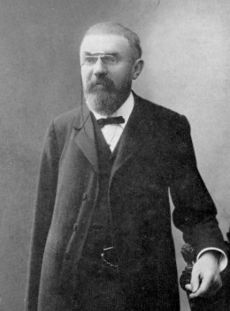
\includegraphics[height=\the\HauteurDesPhotos]{Poincare2}&
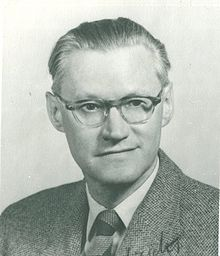
\includegraphics[height=\the\HauteurDesPhotos]{Friedrichs}&
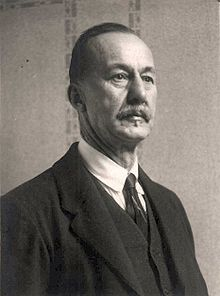
\includegraphics[height=\the\HauteurDesPhotos]{Wirtinger}&
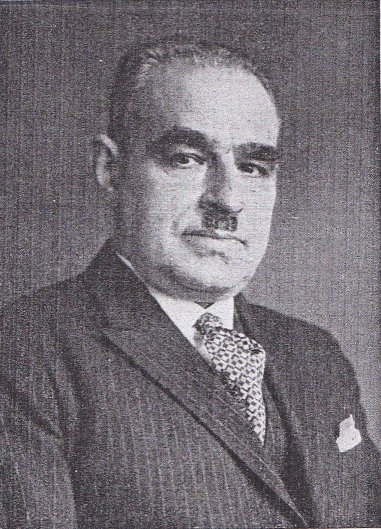
\includegraphics[height=\the\HauteurDesPhotos]{Korn}\\
Poincaré&Friedrichs&Wirtinger&Korn%
\end{tabular}}
\ImageADroite{%
Il est plus connu comme pionnier des télécommunications, plus précisément comme l'inventeur de la téléphotographie. Il met au point un téléautographe, un système de transmission des images fixes à distance, par le biais du fil télégraphique, en recourant aux propriétés photoélectriques du sélénium.}
\end{histoire}

\medskip
\textcolorgreen{%
En mécanique, l'inégalité de Korn\index[aut]{Korn (Arthur), 1870-1945, Allemand} dit que l'énergie élastique (qui est proportionnelle à la norme du tenseur des déformations dans~$L^2(\Omega)$) contrôle (i.e. est supérieure à) la norme du déplacement dans~$H^1(\Omega)$ à l'addition près de la norme du déplacement dans~$L^2(\Omega)$.
Ce dernier point permet de prendre en compte les «mouvements de corps rigides», i.e. les déplacements~$u$ non nuls mais d'énergie élastique nulle.}

